%%%%%%%%%%%%%%%%%%%% author.tex %%%%%%%%%%%%%%%%%%%%%%%%%%%%%%%%%%%
%
% sample root file for your "contribution" to a contributed volume
%
% Use this file as a template for your own input.
%
%%%%%%%%%%%%%%%% Springer %%%%%%%%%%%%%%%%%%%%%%%%%%%%%%%%%%%%%%%

%%%%%%%%%%%%%%%% Remove Warnings, KB#23 %%%%%%%%%%%%%%%%%%%%%%%%%
%\pdfminorversion=10
\RequirePackage{amsmath}
\RequirePackage{mathptmx}
% RECOMMENDED %%%%%%%%%%%%%%%%%%%%%%%%%%%%%%%%%%%%%%%%%%%%%%%%%%%
\documentclass[graybox]{svmult}

% choose options for [] as required from the list
% in the Reference Guide

\usepackage{graphicx, epstopdf}		%changed for windows, KB#23
\usepackage{newtxtext,newtxmath}
%\usepackage{mathptmx}       % selects Times Roman as basic font	%included before \documentclass, KB#23
\usepackage{helvet}         % selects Helvetica as sans-serif font  
\usepackage{courier}        % selects Courier as typewriter font
\usepackage{type1cm}        % activate if the above 3 fonts are
                            % not available on your system

\usepackage{makeidx}        % allows index generation

%\usepackage[dvips]{graphicx}		%commented for epstopdf for windows, KB#23
%\usepackage[dvipdfmx]{graphicx}
%\usepackage{graphicx}      % standard LaTeX graphics tool
                            % when including figure files
\usepackage{graphicx}
\usepackage{comment}
%\usepackage{subfig}
\usepackage{subfigure}
\usepackage{algorithmic}
\usepackage{algorithm}
\usepackage{cite}
\usepackage{svg}
\usepackage{float}
%\usepackage{amsmath}		 %included before \documentclass, KB#23

\usepackage{multicol}        % used for the two-column index
\usepackage[bottom]{footmisc}% places footnotes at page bottom

\def\vector#1{\mbox{\boldmath $#1$}}

% see the list of further useful packages
% in the Reference Guide

\makeindex             % used for the subject index
                       % please use the style svind.ist with
                       % your makeindex program

%%%%%%%%%%%%%%%%%%%%%%%%%%%%%%%%%%%%%%%%%%%%%%%%%%%%%%%%%%%%%%%%%%%%%%%%%%%%%%%%%%%%%%%%%
\begin{document}

\title*{\centering Research Progress Report}

\subtitle{\centering The Development of Haptic Feedback Data Glove for Enhancing Immersion in VR Experiences}
% Use \titlerunning{Short Title} for an abbreviated version of
% your contribution title if the original one is too long
\titlerunning{The Development of Haptic Feedback Data Glove for Enhancing Immersion}
\author{\hfill Korntawat Witchuvanit}
\authorrunning{Korntawat Witchuvanit} 
% your contribution title if the original one is too long
\institute{
     Korntawat Witchuvanit
     \at Graduate School of Engineering, Fukuoka Institute of Technology (FIT), 3-30-1 Wajiro-Higashi, Higashi-Ku, Fukuoka 811--0295, Japan,
     \email{korntawat.contact@gmail.com}
     }


\maketitle

\abstract{In this research progress report, I will present my research for Master's and PhD studies. First, I will introduce the present research related to the development of a wearable haptic glove system for virtual reality applications. The glove integrates flex sensors, motion tracking, and vibration motors to simulate the tactile sensation of different textures. Next, I will present my future research, Next, I will present my future research, which aims to enhance tactile realism by developing a high-resolution tactile display. This system will integrate a dense array of actuators or explore alternative technologies such as piezoelectric elements to achieve more localized and detailed haptic rendering. After that, I will present the detailed plan for each year of my PhD studies. Finally, I will give the conclusions.}

\section{Introduction}
\label{sec:1}

	My Master's studies at FIT are related to the development of a compact and wearable haptic interface for Virtual Reality (VR). Traditional VR controllers can be bulky and restrict natural hand movements, limiting user immersion and tactile perception~\cite{Slater2009, Choi2016}. To address this challenge, we developed a lightweight haptic glove that allows for intuitive hand interaction while delivering tactile feedback through embedded actuators.
	
	The glove integrates flex sensors for finger movement detection, an MPU sensor for tracking hand orientation, and coin-type vibration motors to provide vibrotactile feedback. By applying Pulse Width Modulation (PWM) to control the vibration motors, the system simulates different levels of surface smoothness. In user experiments, participants were able to distinguish between textures rendered at varying PWM cycle rates, indicating that PWM-based feedback can effectively simulate the granularity of virtual textures.
	
	In my Master Thesis, I implemented and evaluated the haptic feedback glove system, confirming its feasibility for realistic texture rendering in VR.


%%%%%%%%%%%%%%%%%%%%%%%%%%%%%%%%%%%%%%%%%%%%%%%%%%%%%%%%%%%%%
%%%%%% Present Research
%%%%%%%%%%%%%%%%%%%%%%%%%%%%%%%%%%%%%%%%%%%%%%%%%%%%%%%%%%%%
\section{Present Research}\label{sec:Present Research}

%%%%%%%%%%%%%%%%%%%% Background and Motivation %%%%%%%%%%%%%%%%%
% \subsection{Background and Motivation}
% As virtual reality (VR) technologies advance, the demand for highly immersive environments that engage multiple sensory modalities continues to grow. While visual and auditory feedback are well-developed, realistic tactile feedback remains a significant challenge in achieving full immersion and embodiment in VR environments~\cite{Slater2009, Choi2016}. Traditional VR controllers often limit natural hand movement and provide limited tactile realism. Therefore, we aimed to develop a compact, wearable haptic glove system that enhances texture perception using vibrotactile feedback.

%%%%%%%%%%%%%%%%%%%% System Overview %%%%%%%%%%%%%%%%%%%%%%%%%%%
\subsection{System Overview}
\label{sec:System Overview}
The proposed wearable haptic device addresses current limitations in natural hand interaction, enhancing texture perception in virtual environments. The system comprises three primary modules: an ESP32 microcontroller, sensory components (flex sensors and IMU), and a coin vibration motor actuator. The detailed architecture of the system is illustrated in Figure~\ref{fig:system_diagram}.

\begin{figure}\centering
	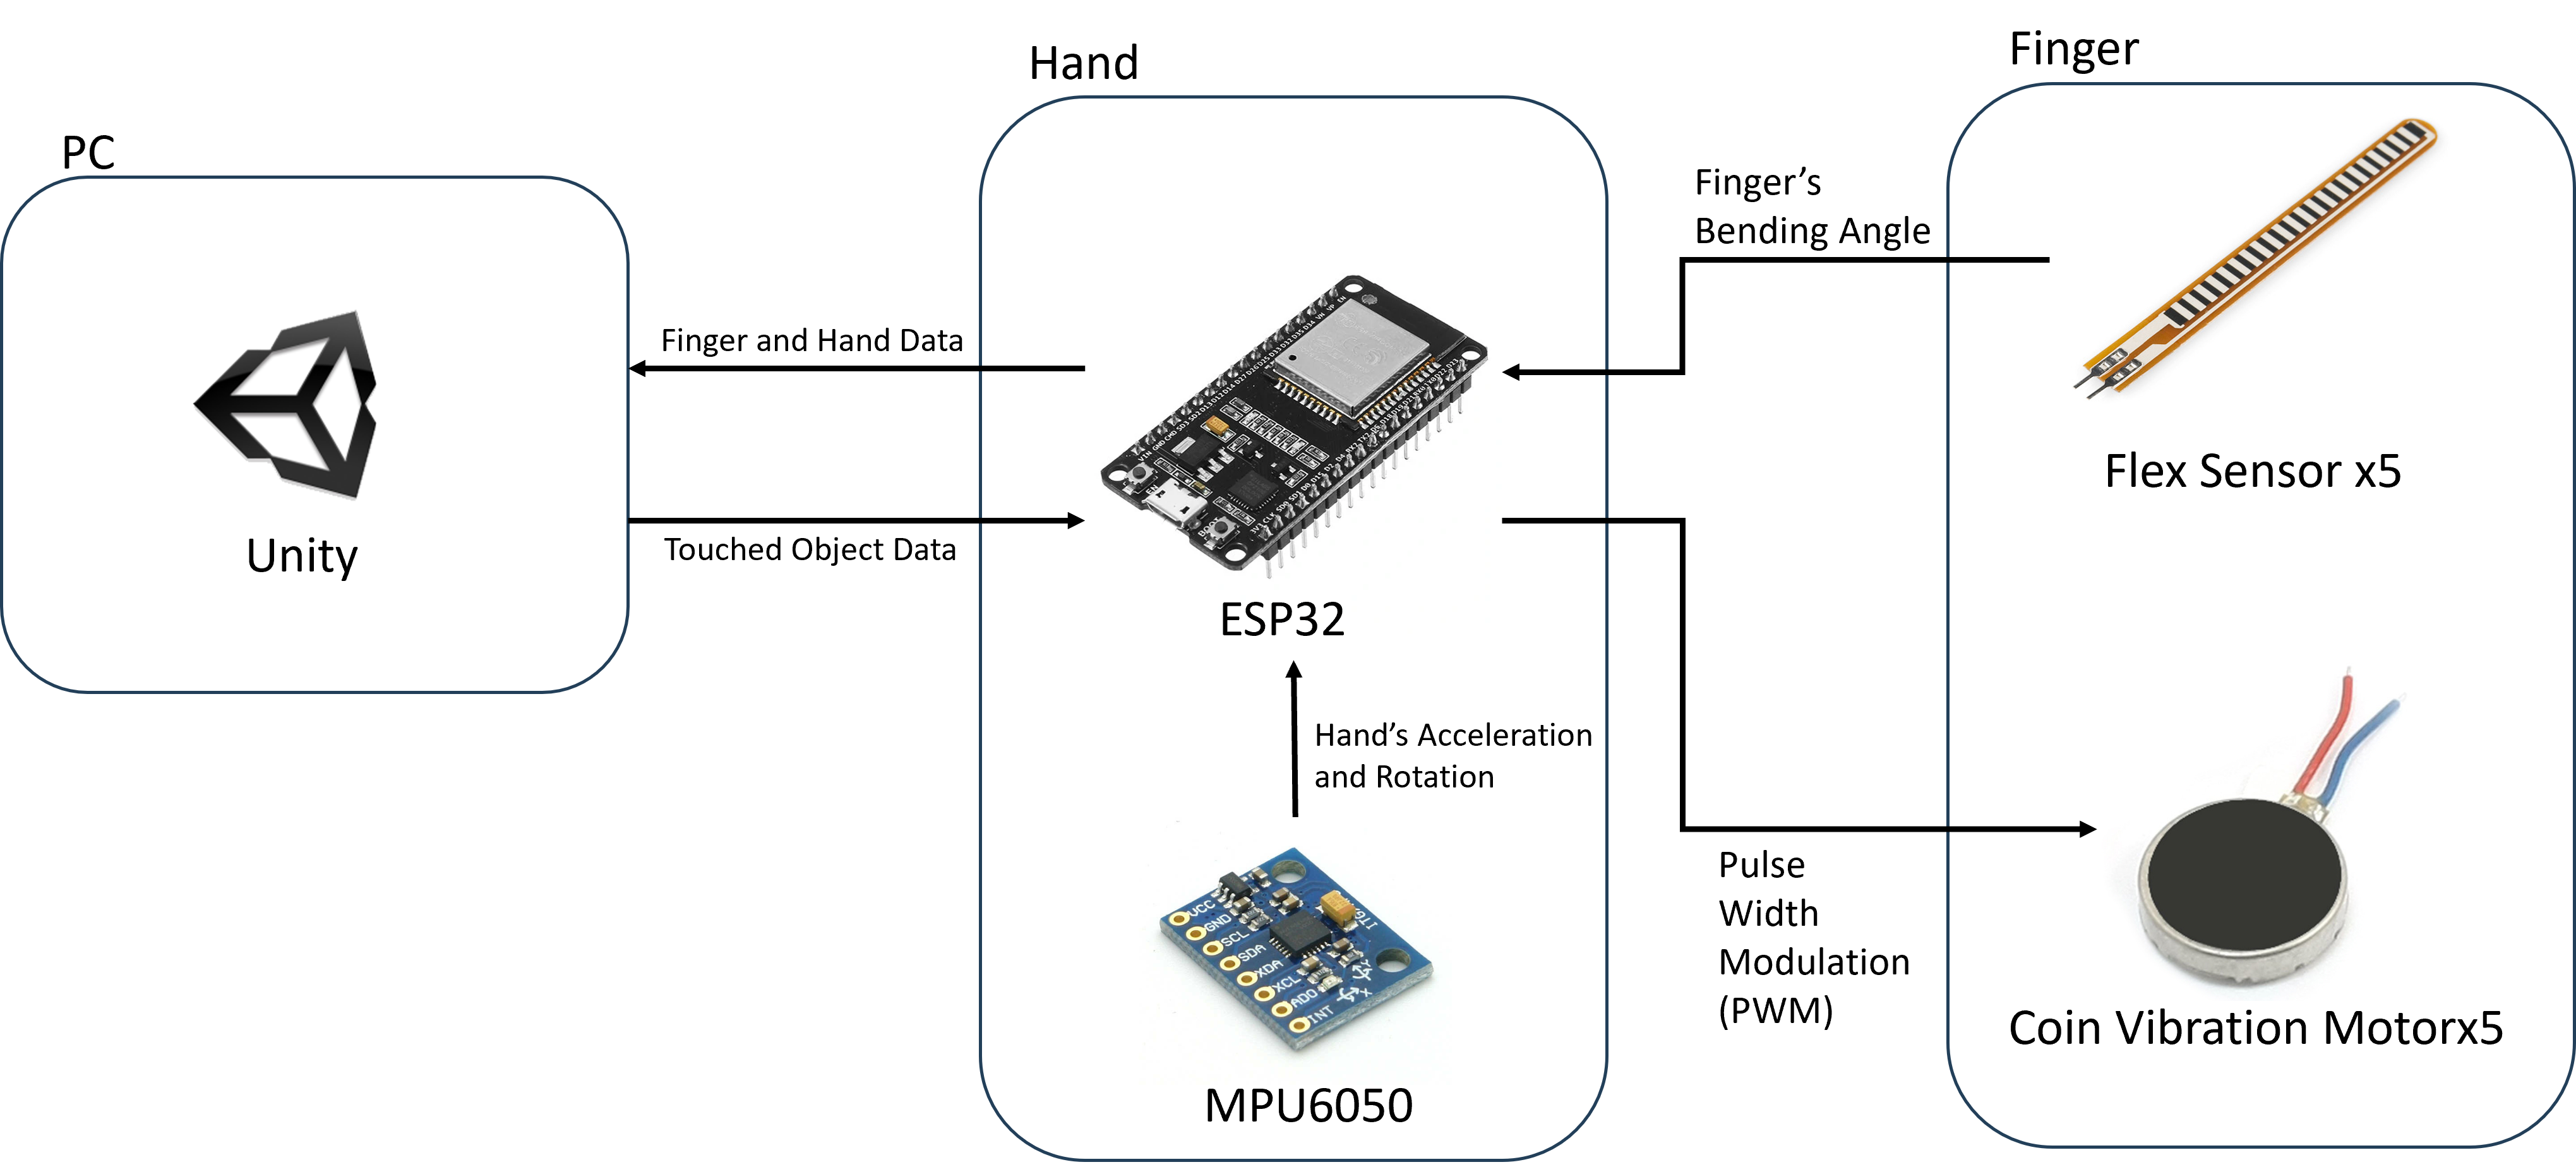
\includegraphics[width=1\textwidth]{figure/system diagram.png}%imagine Avation
	\caption{System architecture of the wearable haptic glove, showing integration between Unity, ESP32, and hardware components.}\label{fig:system_diagram}
\end{figure}
\textbf{ESP32 Microcontroller:}  
The ESP32 functions as the core processing unit, managing sensor data acquisition, real-time data processing, actuator control, and wireless communication. It employs Serial Communication to ensure continuous bidirectional data exchange with Unity, maintaining synchronization of haptic stimuli and sensor readings.

\textbf{Flex Sensors (x5):}  
Five resistive flex sensors, positioned along each finger of the glove, measure finger bending. These sensors deliver real-time analog signals corresponding to finger positions, enabling precise gesture recognition and accurate hand tracking.

\textbf{Inertial Measurement Unit (MPU-6050):}  
An MPU-6050 sensor captures spatial orientation, acceleration, and angular velocity data of hand movements. Integration of IMU measurements enhances spatial coherence between real and virtual hand positions, significantly improving immersive realism and spatial fidelity.

\textbf{Coin Vibration Motor:}  
A coin-type vibration motor generates controlled tactile feedback, utilizing PWM to replicate varying granularities in virtual textures. PWM modulation enables dynamic adjustment of vibration intensity and frequency, simulating realistic sensations from smooth to coarse surfaces. The device provides three distinct haptic feedback, systematically evaluating users' tactile perception sensitivity as recommended by prior research~\cite{strohmeier2017generating, bensmaia2003vibrations}.

The integration of these components into the wearable device is shown in Figure~\ref{fig:glove_1}.

\begin{figure}\centering
	\includegraphics[width=0.5\textwidth]{figure/glove_1.png}%imagine Avation
	\caption{Haptic Data Glove used for texture perception in virtual environments.}\label{fig:glove_1}
\end{figure}

This integrated approach facilitates intuitive interactions in virtual environments, enabling natural hand movements combined with realistic tactile sensations. The selected components directly address limitations noted in existing literature, achieving a lightweight, responsive design with nuanced texture rendering.

%%%%%%%%%%%%%%%%%%%% Experiments %%%%%%%%%%%%%%%%%%%%%%%%%%%
\subsection{Experiments}\label{sec:Experiments}
We conducted two experiments to evaluate the effectiveness of the developed wearable haptic glove. Experiment~1 assessed participants' ability to differentiate among three distinct haptic feedback cycle rates, while Experiment~2 explored the relationship between these cycle rates and the perceived realism of different virtual textures.

Figure~\ref{fig:experiment_setup} shows the general experimental setup, highlighting participant interaction with the haptic glove in the virtual environment.

\begin{figure}\centering
	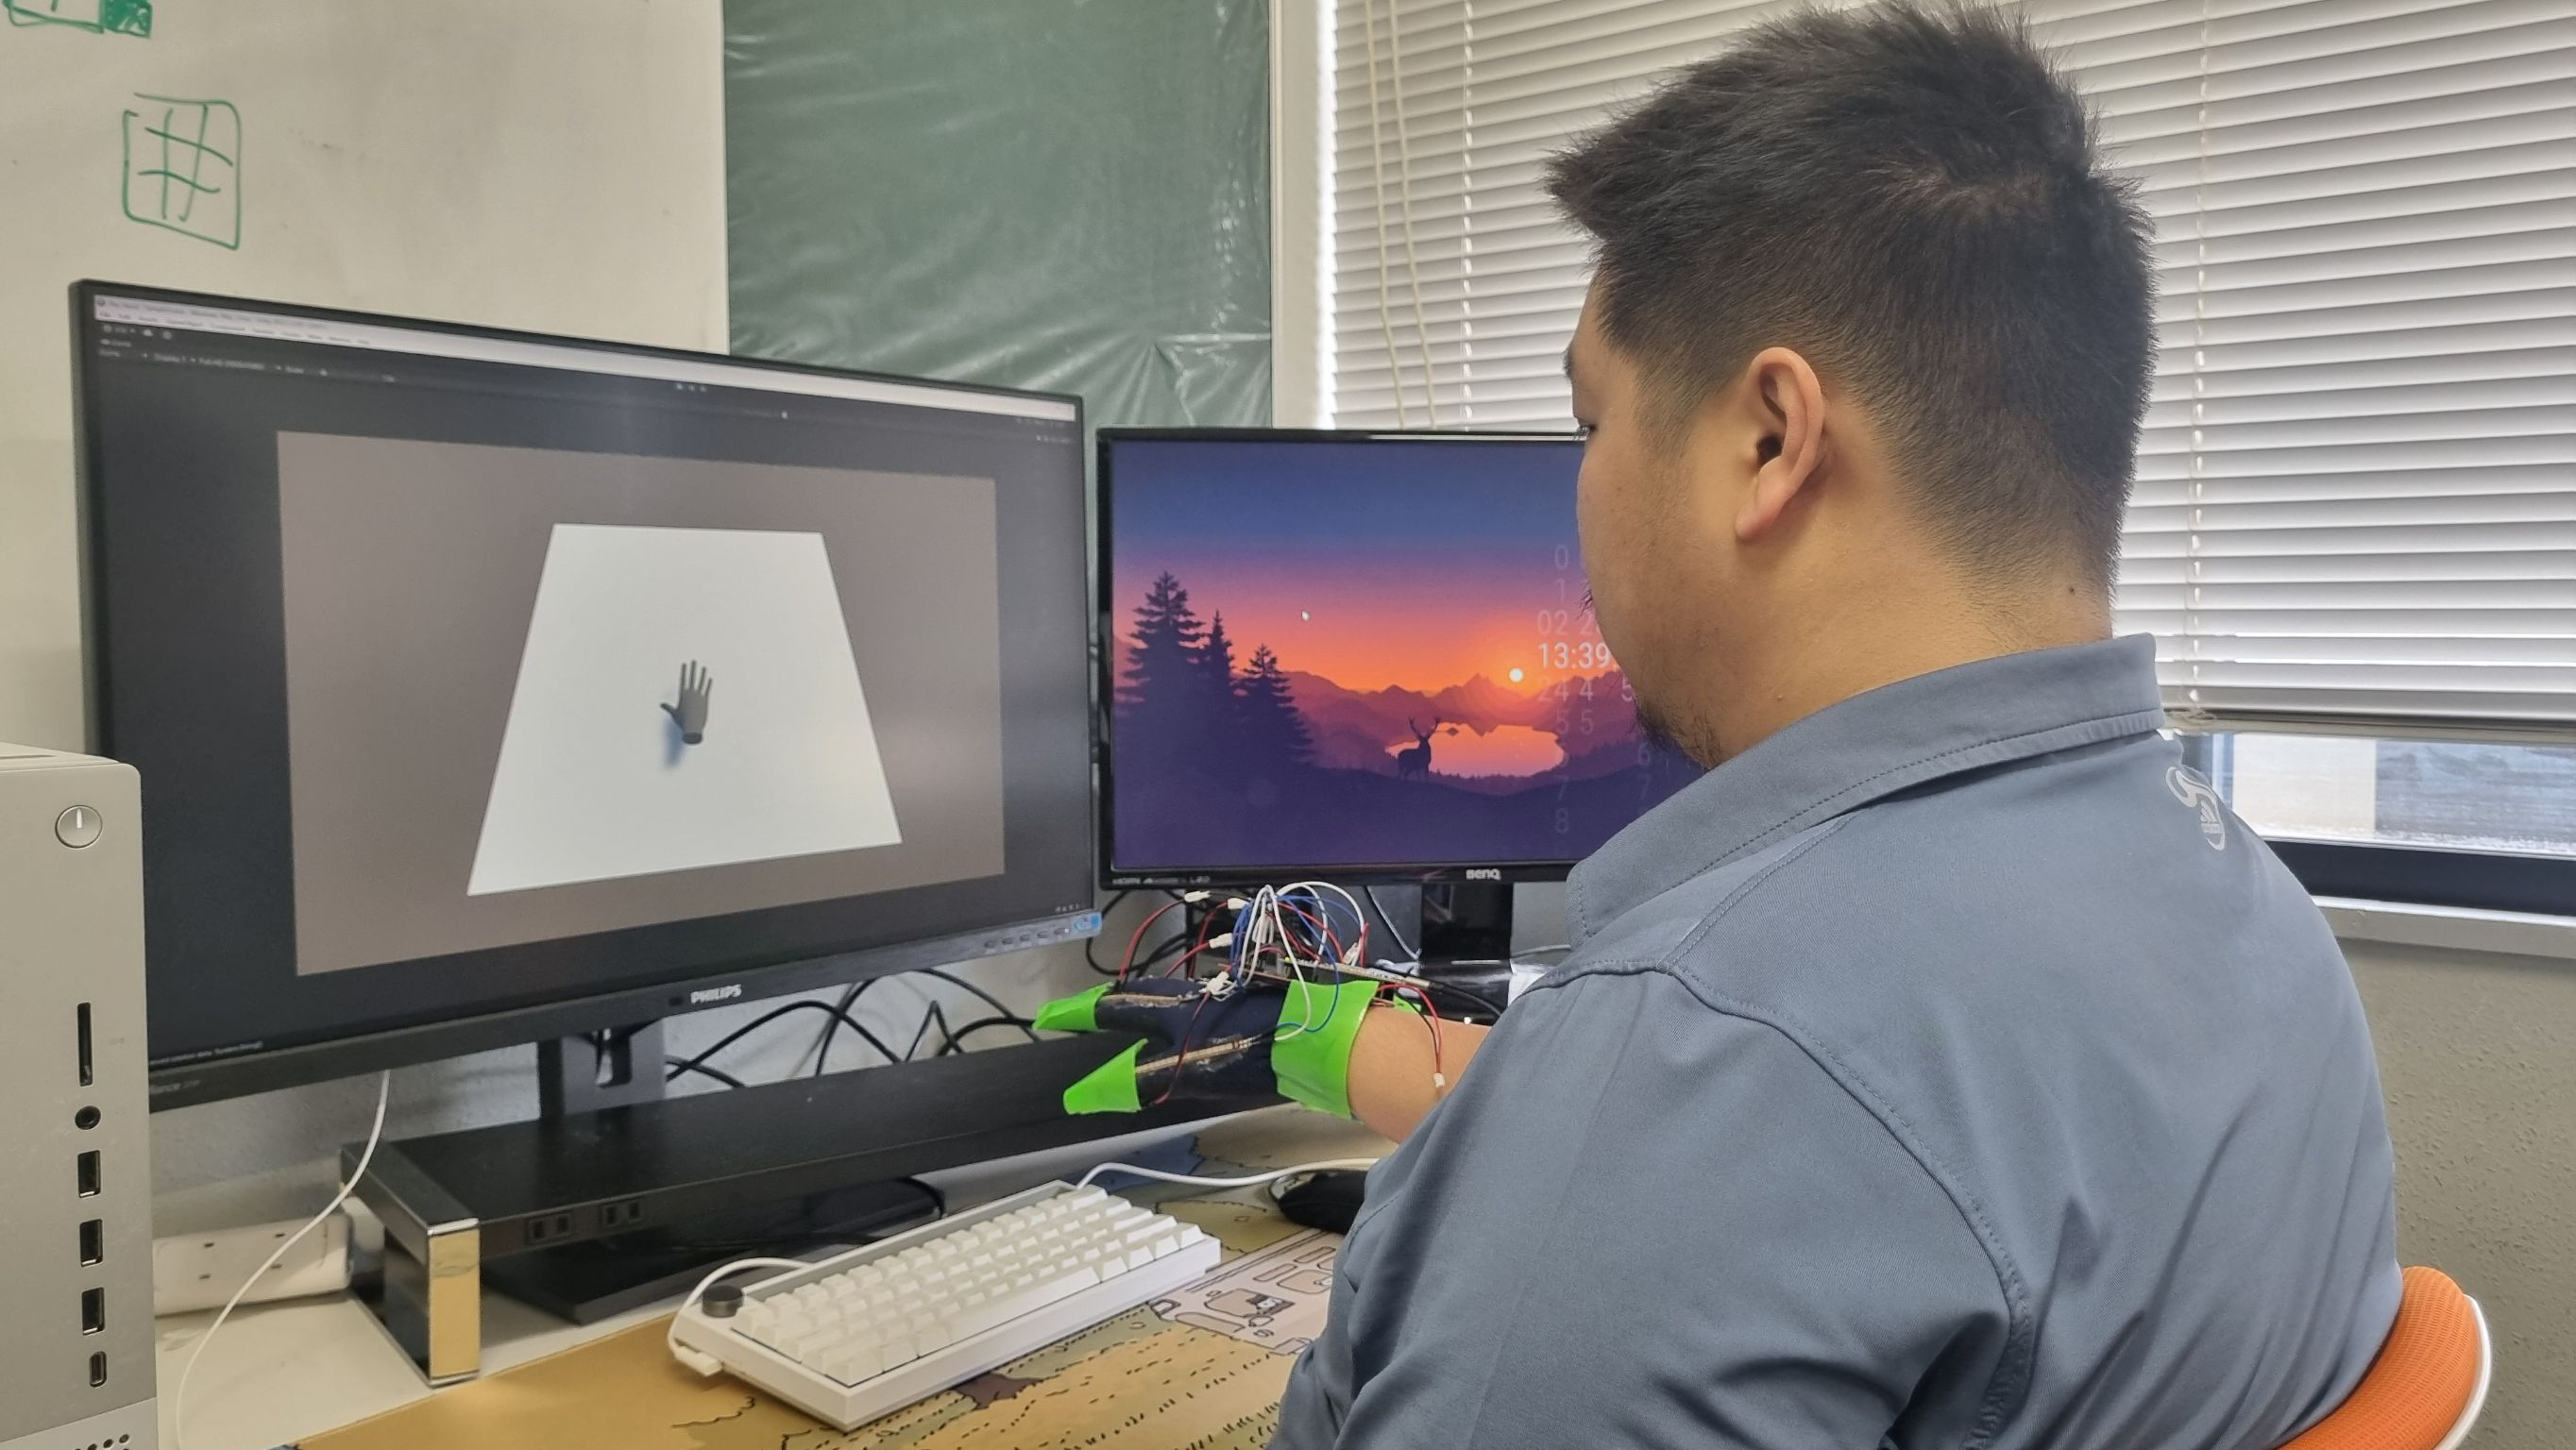
\includegraphics[width=0.7\textwidth]{figure/experiment.png}%imagine Avation
	\caption{Overall experimental setup demonstrating participant interaction using the wearable haptic glove.}\label{fig:experiment_setup}
\end{figure}

\subsubsection{Experiment 1: Distinguishing Haptic Feedback}
We recruited six participants aged 24–27 to performed a blind test to evaluate their ability to distinguish between three distinct vibration cycle rates: 0.2, 0.5, and 1.0. Before starting, participants were familiarized with each cycle rate to establish clear tactile references.
performed a blind test to evaluate their ability to distinguish between three distinct vibration cycle rates: 0.2, 0.5, and 1.0. Before starting, participants were familiarized with each cycle rate to establish clear tactile references.

\textbf{Procedure:} Participants wore and calibrated the glove through repeated hand opening and closing gestures, ensuring accurate hand tracking. Subsequently, participants interacted with a plain white 3D plane in the virtual environment (Figure~\ref{fig:experiment1_setup}), triggering randomly generated vibrations corresponding to one of the three cycle rates. Participants verbally identified the perceived cycle rate after each interaction. Each participant completed 15 randomized trials, assessing their discrimination accuracy.

\begin{figure}[H]
	\centering
	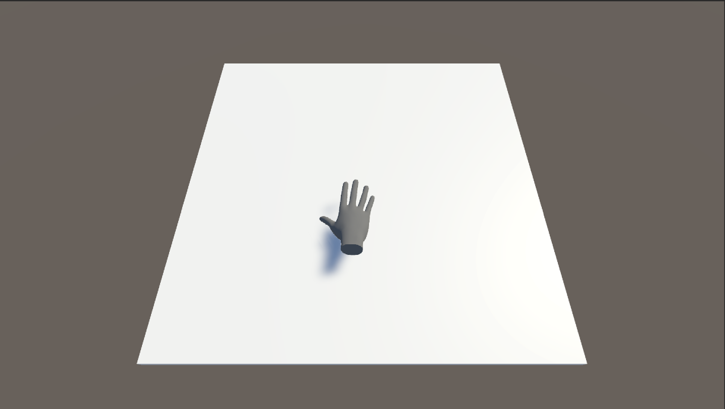
\includegraphics[width=0.7\textwidth]{figure/ex1.png}%imagine Avation
	\caption{Experimental setup for Experiment~1: participants interacting with a plain white virtual plane to distinguish vibration cycle rates.}\label{fig:experiment1_setup}
\end{figure}

\subsubsection{Experiment 2: Relationship Between Haptic Feedback and Texture Perception}
The participants from Experiment 1 were also involved in Experiment 2. This experiment explored how different vibration cycle rates influenced the perceived realism of virtual textures. Participants interacted with three visually distinct textures—brick, grass, and marble—each sequentially paired with vibration cycle rates of 0.2, 0.5, and 1.0.

\textbf{Procedure:} After the first experiment, participants took a 5-minute break before proceeding to the second experiment. In this phase, participants sequentially interacted with each virtual texture (Figure~\ref{fig:experiment2_setup}), experiencing all three vibration cycle rates (0.2, 0.5, and 1.0). After experiencing each set of cycle rates for a given texture, participants selected the cycle rate they felt most accurately matched the visual texture. This procedure was repeated for each texture type, with the order of textures presented randomly for each participant.

\begin{figure}[H]
	\centering
	\includegraphics[width=1\textwidth]{figure/ex2.png}%imagine Avation
	\caption{Experimental setup for Experiment~2: participants interacting with textured virtual planes (brick, grass, marble) to assess vibration realism.}\label{fig:experiment2_setup}
\end{figure}

Collectively, these experiments provided insights into participants' perceptual sensitivity to different vibration cycle rates and evaluated the realism of tactile sensations corresponding to varied virtual textures.

\subsubsection{Post-Experiment Evaluation}
After completing both experiments, participants provided subjective feedback through a questionnaire consisting of 12 statements (Table~\ref{tab:evaluation_questions}). Each statement was rated on a Likert scale from 1 (strongly disagree) to 7 (strongly agree), covering virtual hand embodiment, tactile realism, and immersion. Questions about the sense of virtual hand ownership and control (e.g., Q1, Q3, Q4, Q8) were based on the Virtual Embodiment Questionnaire (VEQ)~\cite{roth2017alpha}. Statements assessing how realistic and aligned the tactile sensations felt (Q2, Q6, Q7, Q10) were guided by the Haptic Experience (HX) model~\cite{schneider2017haptic}. Additionally, overall immersion (Q12) was evaluated according to concepts from the Presence Questionnaire (PQ)~\cite{witmer1998measuring}.

\begin{table}[htbp]
    \centering
    \caption{Post-experiment evaluation questionnaire.}
    \label{tab:evaluation_questions}
    \resizebox{\textwidth}{!}{
    \begin{tabular}{c | c}
        \hline
        \textbf{Question} & \textbf{Statement}\\
        \hline
        Q1 & I felt as if the virtual hands were my own.\\\hline
        Q2 & I felt that the tactile sensations were caused by the virtual hand.\\\hline
        Q3 & I felt as if my hand were the virtual hand.\\\hline
        Q4 & I felt like I was controlling the movement of the virtual hand.\\\hline
        Q5 & I felt as if the virtual hand was naturally connected to my body.\\\hline
        Q6 & The tactile sensations I perceived felt naturally aligned with the virtual hand.\\\hline
        Q7 & When I touched the virtual plane, I felt as if my real hand was also being touched.\\\hline
        Q8 & The movements of the virtual hand felt natural to me.\\\hline
        Q9 & I felt that the virtual hand responded as expected to my movements.\\\hline
        Q10 & I had the sensation that I could feel the texture of objects through the virtual hand.\\\hline
        Q11 & I felt a mismatch between my real hand and the virtual hand.\\\hline
        Q12 & The overall experience made me feel immersed in the virtual environment.\\
        \hline
    \end{tabular}}
\end{table}

Participant responses provided qualitative insights into embodiment, tactile realism, and immersion, complementing the quantitative outcomes from Experiments~1 and 2.

\subsubsection{Results}
\textbf{Experiment 1: Distinguishing Haptic Feedback: }  
Participants' accuracy in identifying the three PWM cycle rates (0.2, 0.5, and 1.0) is summarized in Figure~\ref{fig:ex1_results}. The highest accuracy (26/30) was achieved at the 1.0 cycle rate, suggesting that participants found higher-intensity vibrations easier to identify. Accuracy slightly decreased at lower cycle rates (0.5: 24/30; 0.2: 23/30), indicating that subtler vibrations were more challenging to distinguish. This aligns with prior research indicating that higher vibration intensities yield clearer tactile distinctions~\cite{strohmeier2017generating,bensmaia2003vibrations}. These findings confirm the effectiveness of PWM cycle rates in distinguishing tactile sensations.
\begin{figure}\centering
	\includesvg[width=0.7\textwidth, inkscapelatex=true]{figure/ex1_result}
	\caption{Participants' accuracy in identifying different vibration cycle rates.}\label{fig:ex1_results}
\end{figure}

\textbf{Experiment 2: Relationship Between Haptic Feedback and Texture Perception: }
Participants' preferences for associating specific vibration cycle rates with virtual textures (brick, grass, marble) are illustrated in Figure~\ref{fig:ex2_results}. The marble texture was unanimously associated with the highest cycle rate (1.0), suggesting participants perceived smoother and more rigid textures as best represented by higher-intensity vibrations. Conversely, the brick and grass textures elicited preferences for lower and intermediate cycle rates (0.2 and 0.5), reflecting participants' association of moderate vibrations with intermediate texture roughness. These results clearly highlight the link between vibration granularity and perceived realism, reinforcing the importance of tailored tactile feedback for different textures~\cite{otake2022vibrotactile}.
\begin{figure}[H]
	\centering
	\includesvg[width=0.7\textwidth, inkscapelatex=true]{figure/ex2_result}
	\caption{Participants' accuracy in identifying different vibration cycle rates.}\label{fig:ex2_results}
\end{figure}

\textbf{Post-Experiment Evaluation: }
Subjective feedback (Figure~\ref{fig:questionnaire_results}) revealed high ratings in perceived texture realism (Q10; mean=5.33), tactile alignment (Q7; mean=5.00, Q6; mean=4.83), and overall immersion (Q12; mean=4.83). Moderate agreement was found in tactile sensations attributed directly to the virtual hand (Q2; mean=4.83) and control fidelity (Q4; mean=4.17). Lower scores in embodiment and naturalness of hand interactions (Q5; mean=3.17, Q8; mean=3.17) suggest areas needing further refinement. These results reinforce the success of the glove in enhancing tactile feedback realism and immersion, echoing findings from previous wearable haptic studies~\cite{pacchierotti2017wearable}. However, the lower embodiment scores indicate potential improvements in sensor placement or glove calibration procedures to strengthen the perceived naturalness of virtual hand interactions.

\begin{figure}\centering
	\includesvg[width=0.7\textwidth, inkscapelatex=true]{figure/question_result}
	\caption{Participants' accuracy in identifying different vibration cycle rates.}\label{fig:questionnaire_results}
\end{figure}

%\vspace{1000mm}
%%%%%%%%%%%%%%%%%%%% PhD Research %%%%%%%%%%%%%%%%%%%%%%%%%%%
\section{PhD Research}

My PhD research will focus on enhancing the realism of tactile feedback in Virtual Reality (VR) using perception-based techniques with a small number of actuators. The glove system developed during my Master’s studies used PWM to simulate different textures. While this approach was effective for basic texture rendering, it is difficult to produce fine detail due to the limited number of vibration motors. To address this, we aim to develop a system that uses perceptual illusions and optimized feedback patterns to create the feeling of high-resolution textures without adding hardware complexity.

Human perception can be used to enhance haptic feedback in efficient ways. For example, by activating motors in certain time sequences, it is possible to create the illusion of motion or a continuous surface, even when using only a few actuators. This concept is known as perception-based tactile rendering, where the feedback is designed not only based on the physical signal but also how it is interpreted by the user~\cite{Ujitoko2022,Dandu2021}.

The system will use a rule-based or data-driven control method to select the most suitable vibration pattern for each texture. This includes adjusting parameters such as frequency, intensity, duration, and timing of each motor activation. By applying findings from perception studies, we aim to achieve high tactile realism while keeping the system lightweight and energy-efficient~\cite{Kyung2021,Israr2016}.

\section{Future Work and Annual Research Plan}
\label{sec:conc}
My PhD research plan includes the following topics:
\begin{itemize}
	\item Proposal of new parameters for IFACS.
	\item Experiments with IFACS. 
	\item Comparison of simulation results with other systems and research works.
	\item Comparison of simulation results with experimented results.
\end{itemize}

The detailed plan for each year is as follows.
\begin{enumerate}
	\item In the first year, I will deal with following issues.
	\begin{itemize}
		\item Proposal of new parameters for IFACS
		\item Proposal of new parameters for QoS Evaluation.
		\item Implementation of proposed systems. 
		\item Evaluation of proposed systems.
	\end{itemize}
	\item In the second year, I will deal with following issues.
	\begin{itemize}
		\item Experiments with IFACS. 
		\item Comparison between simulation results and experiment result.
		\item Comparison with other research works.
	\end{itemize}
	\item In the last year, I will deal with the following issues.
	\begin{itemize}
		\item Implementation of integrated call admission control and handover for 5G wireless networks.
		\item Writing of PhD Thesis.
	\end{itemize}
\end{enumerate}


\section{Conclusions}
In this report, I presented my research during Master studies. Then, I introduced 5G Wireless Networks, SDN, FL, GAs and PSO as related technologies and approaches for my PhD studies.


\bibliographystyle{ieeetr}
\bibliography{ref}


\end{document}
